
\tikzset{every picture/.style={line width=0.75pt}} %set default line width to 0.75pt        

\begin{tikzpicture}[x=0.75pt,y=0.75pt,yscale=-1,xscale=1]
%uncomment if require: \path (0,432); %set diagram left start at 0, and has height of 432

%Image [id:dp6404601341090801] 
\draw (359.5,218.99) node  {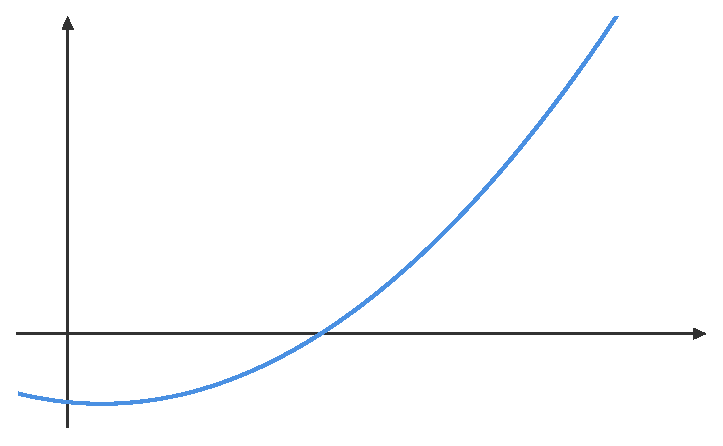
\includegraphics[width=330.75pt,height=197.25pt]{images/image_newton_method}};
%Straight Lines [id:da6424929768444043] 
\draw [color={rgb, 255:red, 155; green, 155; blue, 155 }  ,draw opacity=1 ][line width=0.75]  [dash pattern={on 4.5pt off 4.5pt}]  (510.1,106.5) -- (510.1,284.5) ;
%Straight Lines [id:da8758554517093697] 
\draw [color={rgb, 255:red, 155; green, 155; blue, 155 }  ,draw opacity=1 ]   (510.1,105.5) -- (382,289.33) ;
%Straight Lines [id:da8632115968328404] 
\draw [color={rgb, 255:red, 155; green, 155; blue, 155 }  ,draw opacity=1 ][line width=0.75]  [dash pattern={on 4.5pt off 4.5pt}]  (382,262.5) -- (382,285.33) ;
%Straight Lines [id:da10976638691733442] 
\draw [color={rgb, 255:red, 155; green, 155; blue, 155 }  ,draw opacity=1 ]   (340.5,289.5) -- (382,253.2) ;
%Straight Lines [id:da28590987584360095] 
\draw    (510.1,289.5) -- (510.1,293.2) ;
%Straight Lines [id:da06729921605109834] 
\draw    (510.1,286) -- (510.1,290) ;
%Straight Lines [id:da18775137309121925] 
\draw [color={rgb, 255:red, 155; green, 155; blue, 155 }  ,draw opacity=1 ]   (518.35,93.95) -- (510.1,105.5) ;
%Shape: Circle [id:dp7916165248356848] 
\draw  [fill={rgb, 255:red, 255; green, 255; blue, 255 }  ,fill opacity=1 ] (508.1,105.5) .. controls (508.1,104.4) and (509,103.5) .. (510.1,103.5) .. controls (511.2,103.5) and (512.1,104.4) .. (512.1,105.5) .. controls (512.1,106.6) and (511.2,107.5) .. (510.1,107.5) .. controls (509,107.5) and (508.1,106.6) .. (508.1,105.5) -- cycle ;
%Straight Lines [id:da1316603229735085] 
\draw    (382,289.5) -- (382,293.2) ;
%Straight Lines [id:da9560432424659024] 
\draw    (340.5,289.5) -- (340.5,293.2) ;
%Straight Lines [id:da2626747830873235] 
\draw    (382,286) -- (382,290) ;
%Straight Lines [id:da9507317011882577] 
\draw    (340.5,285.5) -- (340.5,289.5) ;
%Straight Lines [id:da6325259503800027] 
\draw [color={rgb, 255:red, 155; green, 155; blue, 155 }  ,draw opacity=1 ]   (382,253.2) -- (423.5,216.9) ;
%Shape: Circle [id:dp23034405156952054] 
\draw  [fill={rgb, 255:red, 255; green, 255; blue, 255 }  ,fill opacity=1 ] (380,253.2) .. controls (380,252.1) and (380.9,251.2) .. (382,251.2) .. controls (383.1,251.2) and (384,252.1) .. (384,253.2) .. controls (384,254.3) and (383.1,255.2) .. (382,255.2) .. controls (380.9,255.2) and (380,254.3) .. (380,253.2) -- cycle ;
%Straight Lines [id:da641645989007537] 
\draw [color={rgb, 255:red, 155; green, 155; blue, 155 }  ,draw opacity=1 ]   (526.6,82.4) -- (518.35,93.95) ;

% Text Node
\draw (162,68.4) node [anchor=north west][inner sep=0.75pt]  [font=\footnotesize]  {$f( x)$};
% Text Node
\draw (503.5,298.4) node [anchor=north west][inner sep=0.75pt]  [font=\footnotesize]  {$x_{0}$};
% Text Node
\draw (375.5,298.4) node [anchor=north west][inner sep=0.75pt]  [font=\footnotesize]  {$x_{1}$};
% Text Node
\draw (585,285.4) node [anchor=north west][inner sep=0.75pt]  [font=\footnotesize]  {$x$};
% Text Node
\draw (334,298.4) node [anchor=north west][inner sep=0.75pt]  [font=\footnotesize]  {$x_{2}$};
% Text Node
\draw (524,106) node [anchor=north west][inner sep=0.75pt]  [font=\footnotesize,color={rgb, 255:red, 155; green, 155; blue, 155 }  ,opacity=1 ] [align=left] {Curve tangent\\at point $\displaystyle x_{0}$.};
% Text Node
\draw (304,209) node [anchor=north west][inner sep=0.75pt]  [font=\footnotesize,color={rgb, 255:red, 155; green, 155; blue, 155 }  ,opacity=1 ] [align=left] {Curve tangent\\at point $\displaystyle x_{1}$.};


\end{tikzpicture}

